	\index{PSHA!Input model}
An OpenQuake PSHA input model contains three distinct information blocks organised in two main objects: the Source System and the GMPEs System. 

These information blocks include: (1) data regarding location, geometry, and seismicity properties of seismic sources, (2) details about ground motion prediction equations to be  adopted in the calculation, (3) information about the epistemic uncertainties related to the two aforementioned points. A fourth separate, but important, chunk of information being part of the input are calculation settings.

OpenQuake PSHA input models are always defined using two logic tree structures where properties are specified branching level by branching level. In particular, OpenQuake requires two logic-tree structures, one describing epistemic uncertainties associated with the creation of the ERF - called Seismic Source logic tree - 
	\index{Logic Tree!Seismic source}
and one considering the uncertainties connected with the use of GMPEs - called GMPE logic tree. 
	\index{Logic Tree!Ground Motion Prediction Equations}
In cases when epistemic uncertainties are non accounted for, the logic tree structure simply consists of one branching level with just one branch (with weight equal to 1).
%
Further explanations about the way we describe and model logic-trees are provided in section \ref{hazard:logic_tree} at page \pageref{hazard:logic_tree}. 

OpenQuake currently support four types of seismic sources. The description of their main properties - subdivided into source location and geometry and source frequency-magnitude distribution - is provided in Section \ref{hazard:seismic_source_types}. 

The selection of ground motion prediction equations (GMPE) in OpenQuake 
is basically accomplished by specifying a label in a particular file.  
The user can associate a GMPE to each tectonic region considered in the 
analysis (Active Shallow tectonic, Stable Continental etc.). Examples of 
GMPEs selection are provided in section \ref{hazard:gmpe_selection} at page 
\pageref{hazard:gmpe_selection}.

The last, but not less important, block of information characterizing a PSHA 
input model contains calculations settings i.e. parameters specifying the way calculations must be carried out. 
%
The information to be included in this part of the input is strictly related to the properties of the engine. 
%
Section \ref{hazard:calculation_settings} provides an outlook of the hazard specific calculation setting supported by OpenQuake. 
%
% ------------------------------------------------------------------------------
%
% ------------------------------------------------------------------------------
\section{Logic-tree description}
\label{hazard:logic_tree}
Logic-trees are a tool designed to consider in a systematic manner the 
epistemic uncertainties of models and parameters included in a hazard 
analysis.
% . . . . . . . . . . . . . . . . . . . . . . . . . . . . . . . . . . . > Figure
\renewcommand{\psedge}{\ncdiag[armA=0,angleB=180,armB=1cm]}
\begin{figure}[!hb]
%\fbox{\begin{minipage}{\textwidth}
\hfill \\
\textcolor{blue01}{\emph{Branch set definition}}: \dotfill Simple Fault 
	Dip Angle \\
\textcolor{blue01}{\emph{Branch set uncertainty type}}: \dotfill 
	Absolute values \\
\textcolor{blue01}{\emph{Applies to}}: \dotfill Simple faults \\
\textcolor{blue01}{\emph{Correlated branches}}: \dotfill Yes \\
\hfill \\
	\centering
	\begin{psTree}[treemode=R,levelsep=*2cm]
			{\Tr{ }}
		\begin{psTree}[treemode=R]{
			\Tr{\parbox[b]{4cm}{ value = 30$^\circ$ 
				\newline weight=w$_1$}}}%
		\end{psTree}%
		\begin{psTree}[treemode=R,treenodesize=1cm]{
			\Tr{\parbox[b]{4cm}{ value = 45$^\circ$ 
				\newline weight=w$_2$}}}%
		\end{psTree}%
		\begin{psTree}[treemode=R]{
			\Tr{\parbox[b]{4cm}{ value = 60$^\circ$ 
				\newline weight=w$_3$}}}%
		\end{psTree}%
	\end{psTree}%
\\ \hfill \\
%\end{minipage}} % End of fbox
\caption{An example of branch set used to account for the epistemic 
uncertainties on faults dip angle; in this case each branch contains a value 
of the dip.}
\label{fig:logic_tree_branching_levels}
\end{figure}
% . . . . . . . . . . . . . . . . . . . . . . . . . . . . . . . . . . . < Figure
%
\index{Logic Tree!Branch set}
A logic tree cont\-ains three main elements:
\begin{itemize}
\item Branching Level
\item Branch Set
\item Branch
\end{itemize}
%
A branching level expresses the distance from the root of the logic tree of a 
given element of a logic tree structure; in the simplest case each branching 
level corresponds to a single type uncertainty
(e.g. maximum magnitude). 
Indicatively, we can say that the larger the number of branching levels in a 
logic structure the larger is its complexity.
%
A branch set describes an uncertainty model (for example - as previously 
mentioned - a model accounting for the epistemic uncertainties connected with 
the definition of maximum magnitude), composed of a number of mutually 
exclusive and collectively exhaustive options. 
%
Finally, a branch represent a particular alternative in a branch set and 
therefore it refers to an uncertainty model and has a weight expressing - 
according to different interpretations available in the literature 
- ``probabilities or simply subjective indications of relative merit'' 
\citep[][page 999]{bommer2008}.
	\index{Logic Tree!Branch}

%
In more detail, a branch set - the fundamental component in our logic tree data 
model - consists on (1) the parameter (or model) affected 
by uncertainty, (2) the specification of the type of uncertainty (3) the 
listing of the - mutually exclusive and collectively exhaustive 
\citep{bommer2008} - alternative hypotheses (4) a weight for each hypothesis, 
(5) a flag specifying if the branches are (totally) correlated and, (6) the 
index of the branches of the previous level - or the subset of seismic 
sources - to which this branch set applies.

Figure \ref{fig:logic_tree_branching_levels} depicts a branch 
set fixing epistemic uncertainties on the dip angle of simple 
fault sources. In this case the possible values of the dip are specified
on each branch composing the branching set (i.e. 30, 45 and 60 degrees). This 
means that these three values are the only ones admitted for all the sources 
included in the initial seismic source model considered. 
%
Figure \ref{fig:logic_tree_branching_levels_1} also shows a branch
set defining epistemic uncertainties on the dip angle 
of simple fault sources. In this case, however, the values specified for each 
branch aren't absolute dip angles but instead differential values to be added - 
or subtracted - to the initial dip value specified for each simple fault source 
contained in the initial seismic sources model.

% ..............................................................................
% . . . . . . . . . . . . . . . . . . . . . . . . . . . . . . . . . . . > Figure
\renewcommand{\psedge}{\ncdiag[armA=0,angleB=180,armB=1cm]}
\begin{figure}
%\fbox{\begin{minipage}{\textwidth}
\hfill \\
\textcolor{blue01}{\emph{Branch set definition}}: \dotfill
	Simple Fault Dip Angle \\
\textcolor{blue01}{\emph{Branch set uncertainty type}}: \dotfill
	Relative values \\
\textcolor{blue01}{\emph{Applies to}}: \dotfill
	All previous branches \\
\textcolor{blue01}{\emph{Correlated branches}}: \dotfill Yes \\
\hfill \\
	\centering
	\begin{psTree}[treemode=R,levelsep=*2cm]
			{\Tr{ }}
		\begin{psTree}[treemode=R]{
			\Tr{\parbox[b]{4cm}{ value = -15$^\circ$ 
				\newline weight=w$_1$}}}%
		\end{psTree}%
		\begin{psTree}[treemode=R,treenodesize=1cm]{
			\Tr{\parbox[b]{4cm}{ value = 0$^\circ$ 
				\newline weight=w$_2$}}}%
		\end{psTree}%
		\begin{psTree}[treemode=R]{
			\Tr{\parbox[b]{4cm}{ value = +15$^\circ$ 
				\newline weight=w$_3$}}}%
		\end{psTree}%
	\end{psTree}%
\\ \hfill \\
%\end{minipage}} % End of fbox
\caption{An example of branch set used to account for the epistemic 
uncertainties on faults dip angle; in this case each branch contains a 
differential from a default dip value indicated for each source in the 
initial seismic sources model.}
\label{fig:logic_tree_branching_levels_1}
\end{figure}
% . . . . . . . . . . . . . . . . . . . . . . . . . . . . . . . . . . . < Figure
% ..............................................................................
%
Two or more branch sets they can be combined in flexible fashion (i.e. 
concatenated) to create an entire logic-tree structure.
Figure \ref{fig:logic_tree_schema} shows an example of a logic tree 
created by combining the two branch sets described in the upper part of the
figure. 
The first branching level accounts for epistemic uncertainties connected with 
the dip of simple fault sources whilst the second branching level specifies 
the epistemic uncertainties relative to the depth to the top of rupture for 
(this branching level also applies to simple faults included in the model).

%A logic tree structure can then be assembled by concatenating many 
%branch sets in a sequence, each position in this stack being represented 
%by a branching level (see Figure \ref{fig:LogicTreeGeneralStructure}).
%
% . . . . . . . . . . . . . . . . . . . . . . . . . . . . . . . . . . . > Figure
\begin{figure}
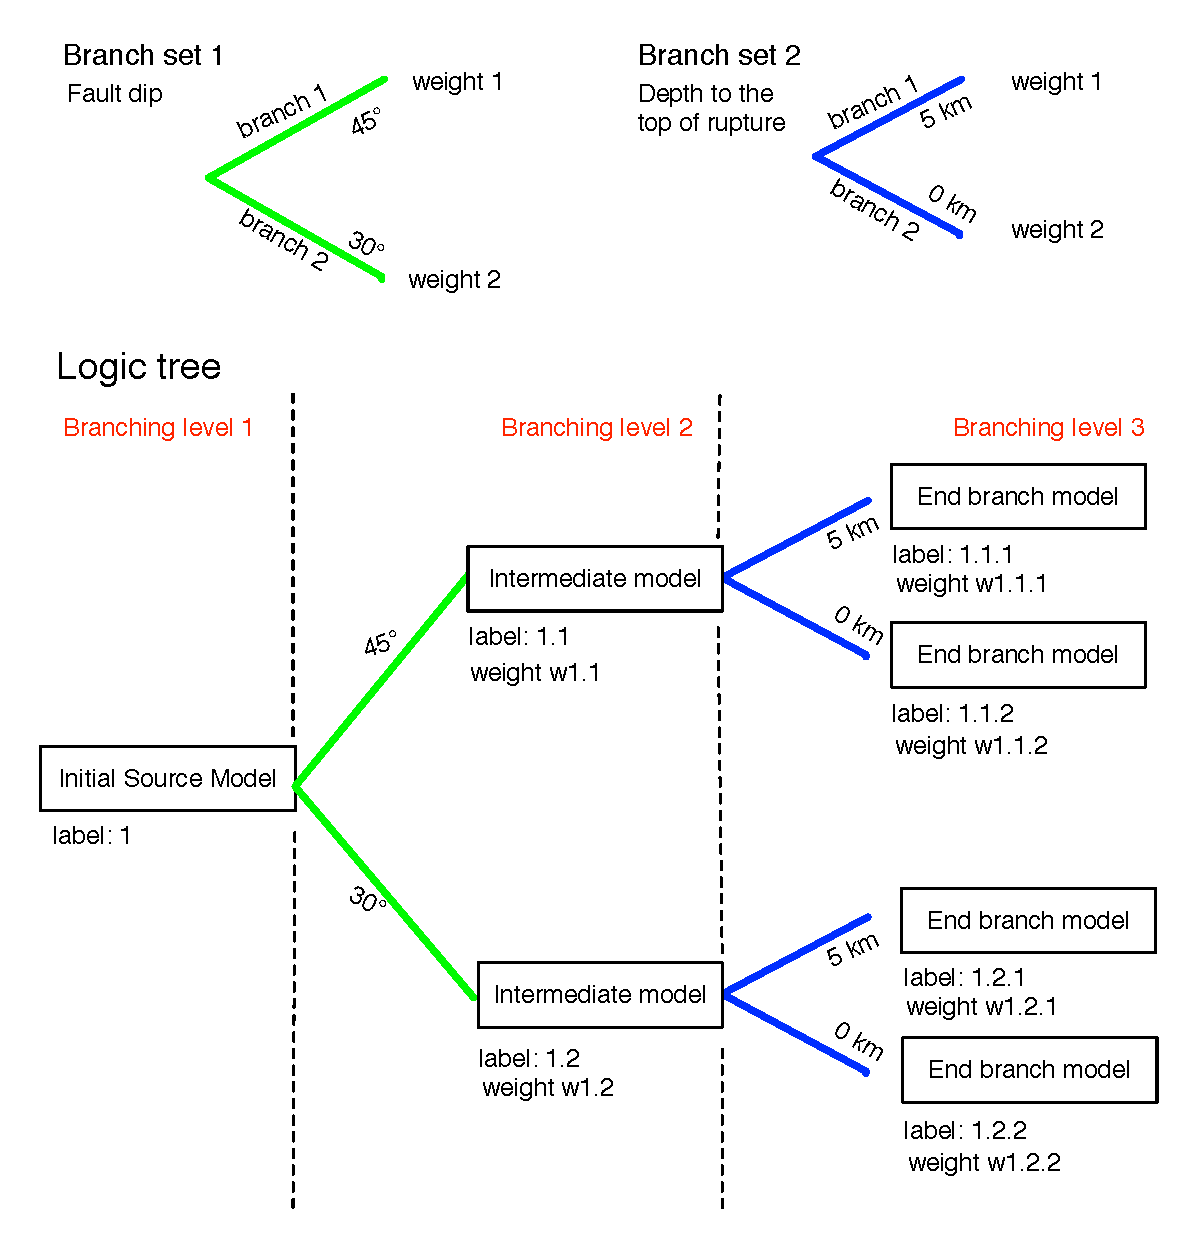
\includegraphics[width=15cm]{./Figures/Part_Hazard/logic_tree_schema.eps}
\caption{Example of a logic tree structure as defined in OpenQuake. The upper
part of the Figure depicts two branch sets.}
\label{fig:logic_tree_schema}
\end{figure}
% . . . . . . . . . . . . . . . . . . . . . . . . . . . . . . . . . . . < Figure
%
We use this logic tree description to specify the structure of the Seismic 
Sources Logic Tree as well as for the Ground Motion Models Logic Tree. 

\clearpage
%===============================================================================
\section{Damiano}
\dotfill \\
%
% ------------------------------------------------------------------------------
\section{Logic-tree description}
\label{hazard:logic_tree}
A logic tree is defined in terms of three main elements:
\begin{itemize}
\item \textbf{Individual Branch}
\item \textbf{Branch Set}
\item \textbf{Branching Level}
\end{itemize}
An individual branch represent a particular realization of an epistemic 
uncertainty, and is therefore defined by an \textbf{uncertainty model} 
and an \textbf{uncertainty weight}. A branch set collects all the individual
branches that describe a particular epistemic \textbf{uncertainty type},
and consequently requires all individual branches' weights to sum to one. 
A logic tree structure can then be assembled by placing branch sets in a 
sequence, each position being represented by a branching level (see Figure 
\ref{fig:LogicTreeGeneralStructure}).
\begin{figure}
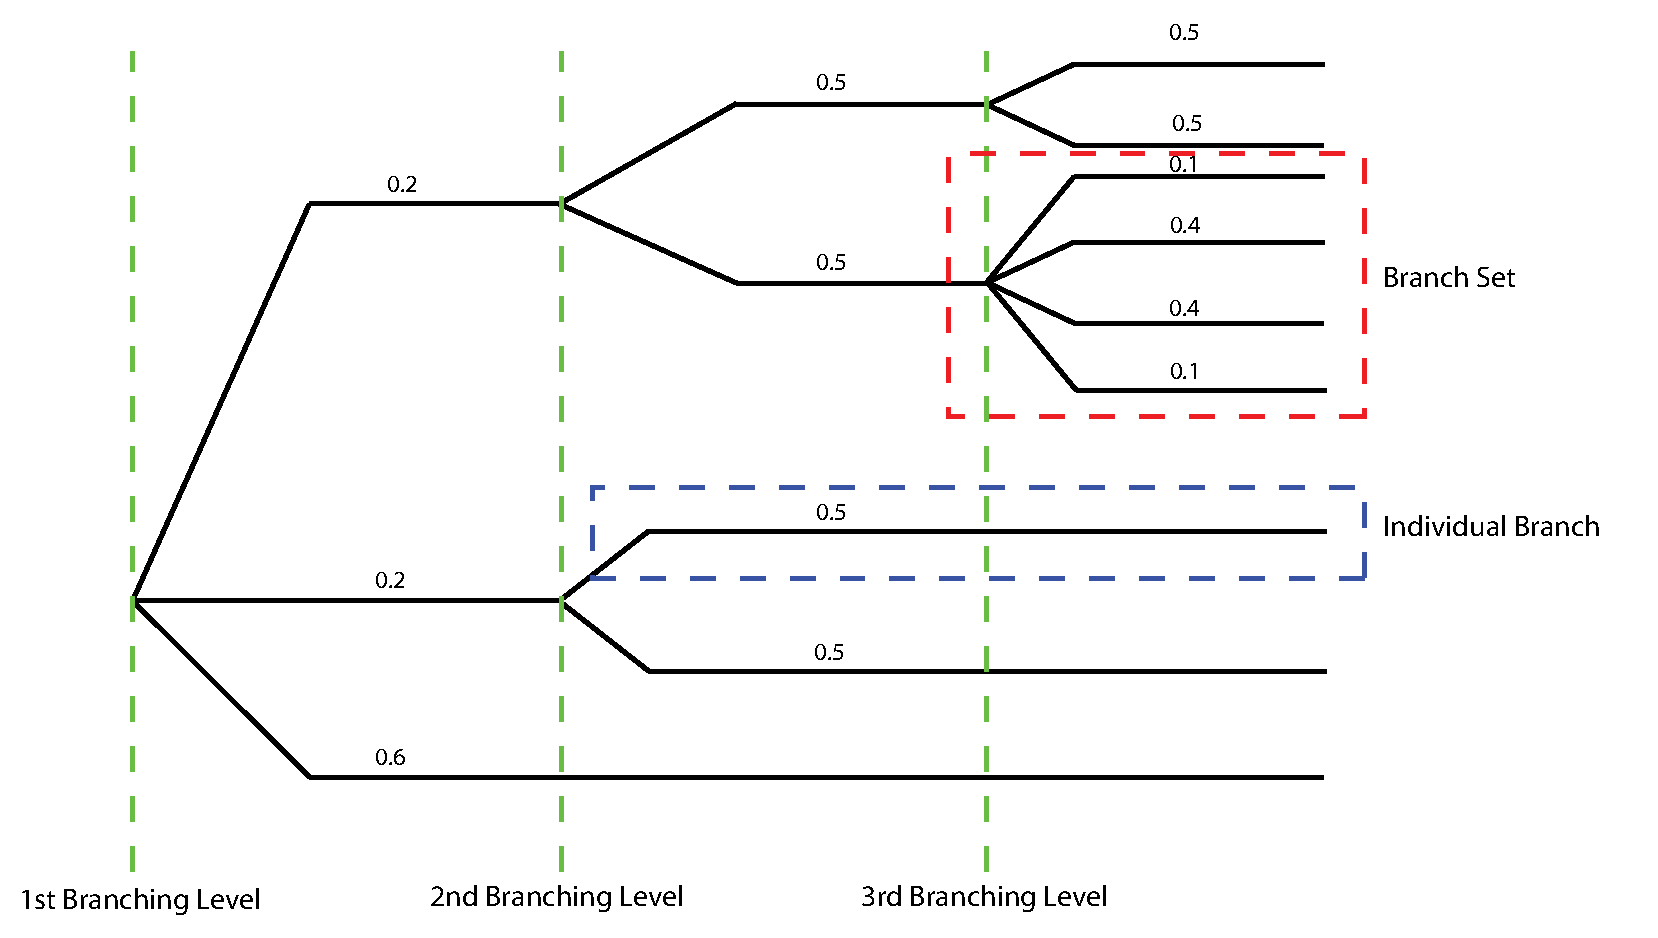
\includegraphics[width=15cm]{./Figures/Part_Hazard/LogicTreeGeneralStructure.eps}
\caption{Logic Tree data structure as defined in terms of individual branches, 
branch sets, and branching levels.}
\label{fig:LogicTreeGeneralStructure}
\end{figure}
The above described parameterization allows for a very general definition of a 
logic tree structure. For instance, a non-symmetric logic tree can be easily 
created by placing multiple branch sets in the same branching level, each 
branch set being connected to a specific branch of a branch set defined in a
previous branching level.
\subsection{Source Model Logic Tree}
\label{hazard:source_model_logic_tree}
In the current version of OpenQuake, a source model logic tree can be defined 
according to the following schema:
\begin{itemize}
\item the 1st branching level is assumed describing one or more "alternative" 
initial source models.
\item subsequent branching levels define source parameters uncertainties. 
Parameters uncertainties are applied independently to each seismic source 
in a source model. That is epistemic uncertainties are assumed uncorrelated 
between different seismic sources.
\item one branch set can be defined for branching level, thus assuming 
symmetric logic tree definition only.
\end{itemize}
The possibility of defining multiple source models in the first branching 
level responds to the need of modern PSHA of considering alternative source 
model creation approaches (as derived by different expert opinions, data sets,
modeling methodologies, for instance). Subsequent branching levels allows 
defining epistemic uncertainties that apply to specific parameters seismic 
sources depends upon. Parameter-related epistemic uncertainties are 
implemented as \textbf{rules}, that is as algorithms describing how 
a certain model parameter has to be altered. The major advantage of 
using a rule-based approach is that a user does not need to a provide 
an input file containing a source model definition corresponding to a 
specific epistemic uncertainty, that is instead computed and applied 
on the fly to the initial model. The current version of OpenQuake offers 
two built-in rules:
\begin{itemize}
\item Gutenberg-Richter b value uncertainties. The user can specify a set 
of increments (positive or negative) that are added to Gutenberg-Richter 
b values. Conservation of total moment rate is assumed.
\item Gutenberg-Richter maximum magnitude uncertainties. The user can specify
a set of increments (positive or negative) that are added to Gutenberg-Richter 
maximum magnitude values. Conservation of total moment rate is assumed.
\end{itemize}
Figure \ref{fig:SourceModelLogicTree} depicts a source model logic tree that 
can be defined with the options currently present in OpenQuake.
%
\begin{figure}
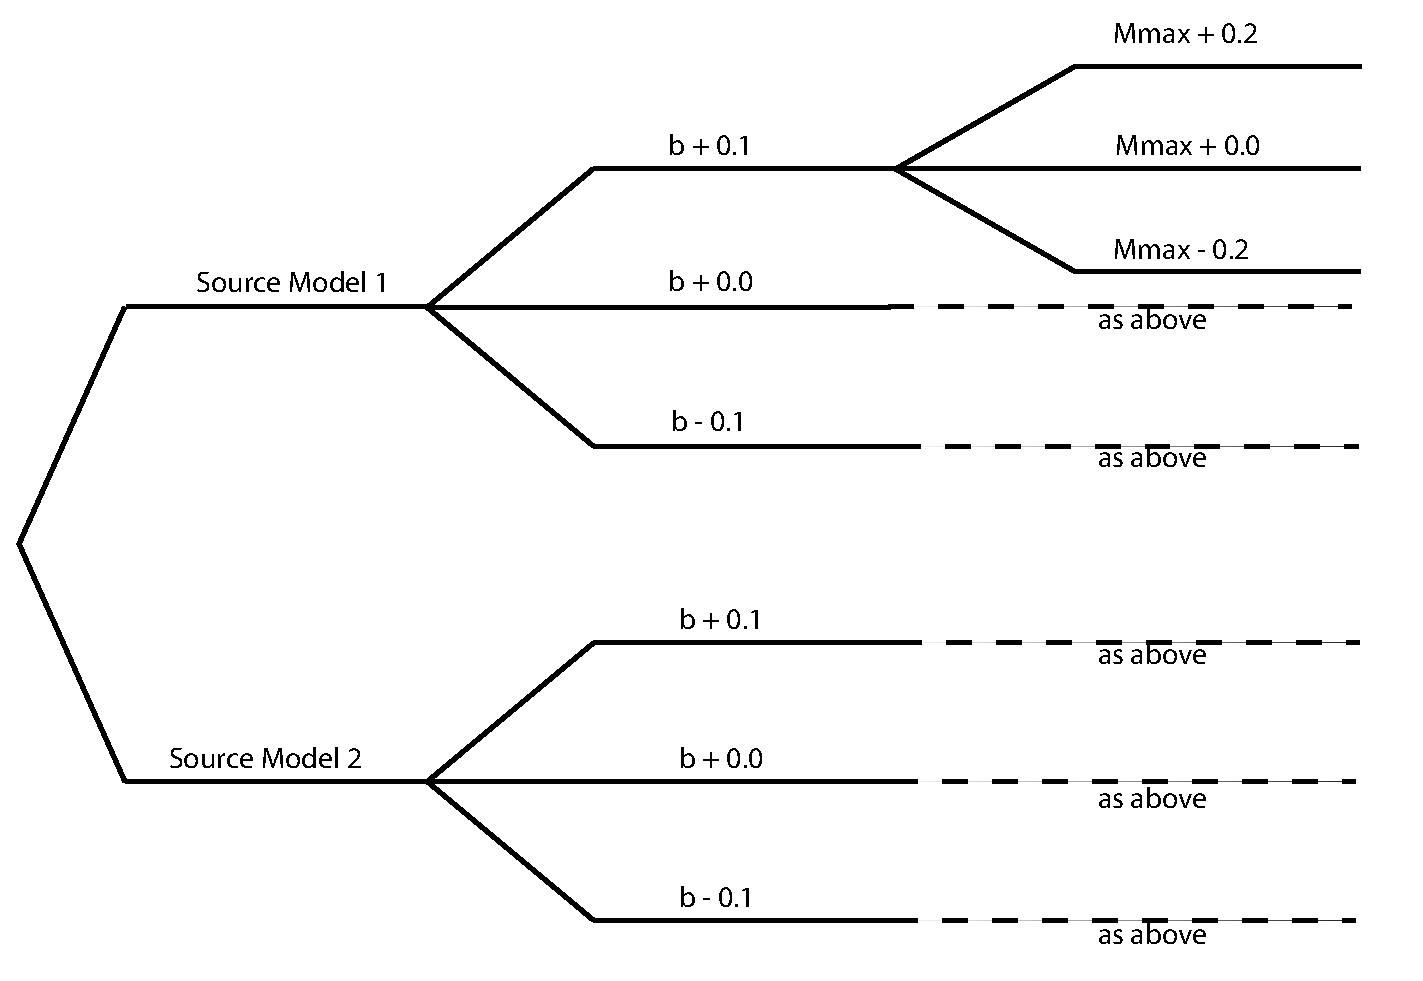
\includegraphics[width=15cm]{./Figures/Part_Hazard/SourceModelLogicTree.eps}
\caption{Example of Source Model Logic Tree. The first branching level defines
two alternative source models (Source Model 1, Source Model 2). The second 
branching level defines uncertainties in b value (increment of 0.1, 0.0, -0.1).
The third branching level defines uncertainties in maximum magnitude 
(increments of 0.2, 0.0, -0.2).}
\label{fig:SourceModelLogicTree}
\end{figure}
%
The above mentioned rules are only a sample of possible source model epistemic 
uncertainties, and future versions of OpenQuake will provide a broader spectrum
of built-in epistemic uncertainties. Currently, rules are applied to all 
sources. Option to apply rules only to specific sources will be also supported 
in the future.
%
\subsection{GMPE Logic Tree}
\label{hazard:gmpe_logic_tree}
The GMPE Logic Tree allows a user to consider multiple ground motion prediction
equations in the hazard modeling. Given that GMPEs are often, or can be, 
associated to specific tectonic region types, OpenQuake allows the definition 
of multiple GMPE logic trees, one for each tectonic region type considered in 
the source model. In the current version, a GMPE logic tree can have only one 
branching level, containing only one branch set, where each individual branch 
is associated to a specific GMPE. With the current setting, epistemic 
uncertainties coming from different models can be taken into account, but 
epistemic uncertainties inside each model cannot be captured.
Figure \ref{fig:GMPELogicTree} schematically shows GMPE logic trees that can 
be currently defined in OpenQuake.
% 
\begin{figure}
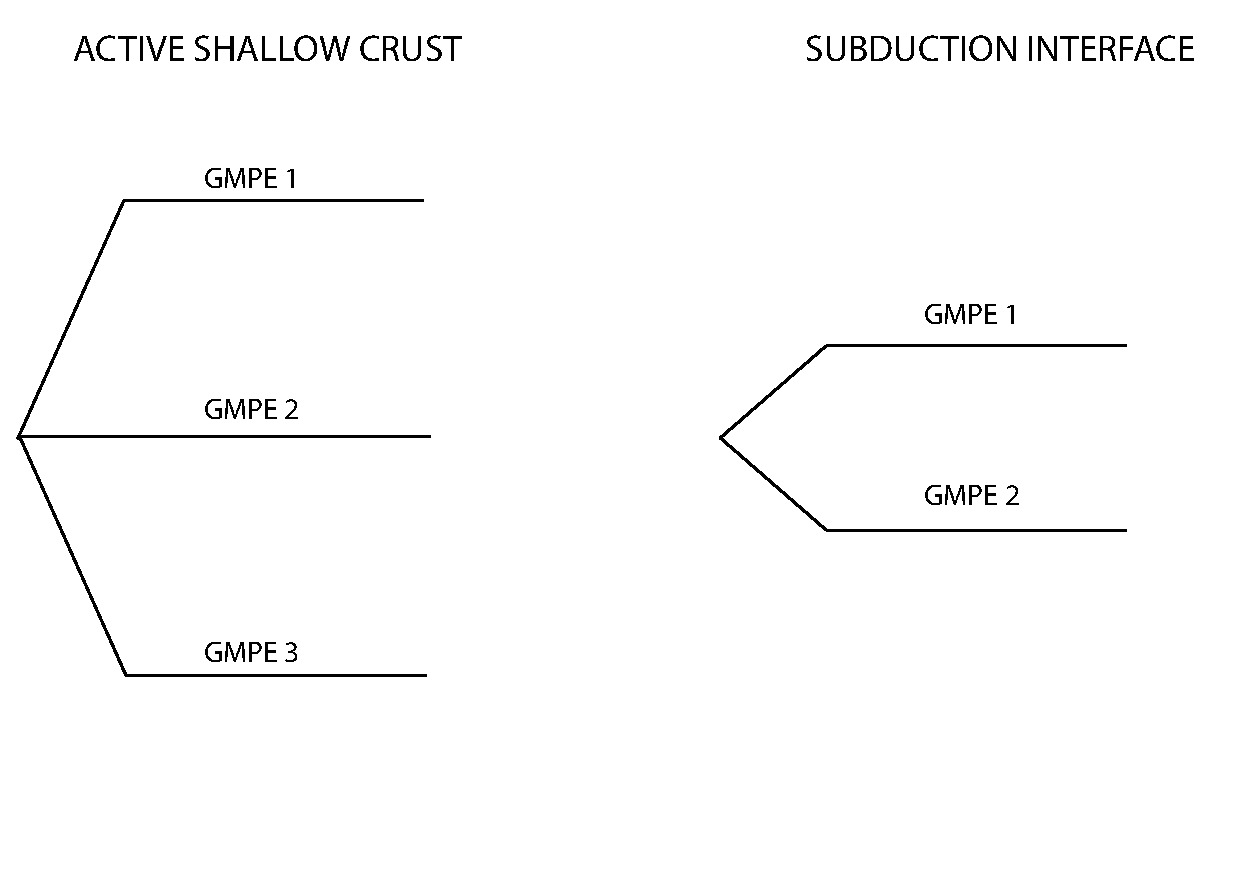
\includegraphics[width=15cm]{./Figures/Part_Hazard/GMPELogicTree.eps}
\caption{Examples of GMPE Logic Trees. One for active shallow crust (considering
three GMPEs) and one for subduction interface (considering two GMPEs).}
\label{fig:GMPELogicTree}
\end{figure}
%
% ------------------------------------------------------------------------------
%
% ------------------------------------------------------------------------------
% ------------------------------------------------------------------------------
\section[OpenQuake seismic source typologies]{OpenQuake seismic source typologies}
%  
A PSHA input model - excluding memory resources constraints - contains an 
unlimited number of sources specified in agreement with the typologies 
supported by OpenQuake.
Each source type supported by OpenQuake is described by a limited numeber 
of parameters; in the following sections we provide a detailed description 
of the source typologies currently supported.
%
%  - - - - - - - - - - - - - - - - - - - - - - - - - - - - - - - - - - - - - - -
\subsection{Seismic source typologies description}
\label{hazard:seismic_source_types}
%
OpenQuake, at present time, provides four seismic source typologies, for the 
most part defined in the course of the GEM1 project \citep{pagani2010}. 
These are:
\begin{itemize}
\item Area source - So far, the most frequently adopted source type in 
national and regional PSHA models.
\item Grid source - Grid sources can be considered a replacement for area 
sources since they both model distributed seismicity;
\item Simple fault sources - Simple faults are the easiest way to
to specify a fault source in OpenQuake. This typology is usually adopted 
to describe shallow seismogenic fault sources.
\item Complex fault sources - Complex faults are habitually adopted to model
subduction interface sources with a complex geometry. 
\end{itemize}

These are the basic assumptions accepted in the definition of these source 
typologies:
\begin{itemize}
\item In the case of area and fault sources, the seismicity is homogeneously 
distributed over the source; 
\item Seismicity temporal occurrence follows a Poissonian model; 
\item The frequency-magnitude distribution can be approximated to an evenly 
discretized distribution. 
\end{itemize}
%
%  . . . . . . . . . . . . . . . . . . . . . . . . . . . . . . . . . . . . . . . 
\subsubsection{Area sources}
\label{hazard:seismic_source_types:areaSources}
\index{Source type!area} 
\index{Area source|see{Source type}}
Area sources model the seismicity occurring over wide areas where fault 
sources identification or characterization - i.e. unambiguous definition 
of seismicity occurrence parameters - is difficult. 

The \citet{sshac1997} defined three main types of area seismic sources using as 
a discriminant their extension:
\begin{enumerate}
\item Area sources enclosing concentrated zones of seismicity;
\item Regional area sources;
\item Background area sources.
\end{enumerate}
The criteria adopted for their definition - and the related uncertainties - vary 
according to each area source type. From a hazard computation standpoint we do 
not introduce any difference between these three area types.
	\marginpar{marco: In the future we may support a specialized background 
	area source type}
%
%  . . . . . . . . . . . . . . . . . . . . . . . . . . . . . . . . . . . . . . . 
\paragraph{Parameters}
\begin{itemize}
\item A polygon that identifies the external border of the area. Eventually, 
internal borders can be specified so as to create holes inside an area
	\textcolor{red}{[The current version of OQ doesn't support the definition 
	of internal borders]}
\item One (or many) combinations of the following objects:
\begin{itemize}
	\item A discrete Frequency-Magnitude Distribution (FMD)
	\item (optional) Strike, dip, and rake angles characterizing the seismicity  
	in the corresponding FMD.
	For example, \cite{coppersmith2009} defines a discrete distribution of 
	strike values (dip is not considered because the source-site metrics they 
	use is the Joyner-Boore distance). 
\end{itemize}
This description permits the accurate characterization of seismicity occurrence 
within an area by explicitly distributing the seismicity on the existing 
faulting trends. 
\item An array specifying the depth to the top of rupture dependency on 
magnitude. The array contains two columns and one or many $<$depth, magnitude$>$ 
tuples. Each tuple specifies the depth to the top of rupture for magnitudes 
equal or greater than the corresponding value. 
\item A value to indicate the hypocentral depth in case of punctual sources. 
By convention all the events with magnitude lower than the lowest value of 
magnitude contained in the depth to the top of rupture array are modelled as 
punctual source. On the opposite, ruptures with magnitude equal or greater than 
the lowest value of magnitude contained in the depth to the top of rupture array 
are modelled considering their finite dimensions. The finite dimension of the 
rupture is computed using a magnitude-area or magnitude-length relationship 
specifies in the calculation settings file (in future versions of OQ we will 
allow the user to specify for each tectonic region the corresponding 
magnitude-scaling relationship).
\end{itemize}
%
%  . . . . . . . . . . . . . . . . . . . . . . . . . . . . . . . . . . . . . . . 
\subsubsection{Multi-depth area sources}
\label{hazard:seismic_source_types:multiDepthAreaSources}
\index{Source type!area multi-depth} 
\index{Multi-depth area source|see{Source type}}
Area sources model the seismicity occurring over wide areas where fault 
sources identification or characterization - i.e. unambiguous definition 
of seismicity occurrence parameters - is difficult. 

The \citet{sshac1997} defined three main types of area seismic sources using as 
a discriminant their extension:
\begin{enumerate}
\item Area sources enclosing concentrated zones of seismicity;
\item Regional area sources;
\item Background area sources.
\end{enumerate}
The criteria adopted for their definition - and the related uncertainties - vary 
according to each area source type. From a hazard computation standpoint we do 
not introduce any difference between these three area types.
	\marginpar{marco: In the future we may support a specialized background 
	area source type}
%
%  . . . . . . . . . . . . . . . . . . . . . . . . . . . . . . . . . . . . . . . 
\paragraph{Parameters}
\begin{itemize}
\item A polygon that identifies the external border of the area. Eventually, 
internal borders can be specified so as to create holes inside an area
	\textcolor{red}{[The current version of OQ doesn't support the definition 
	of internal borders]}
\item One (or many) combinations of the following objects:
\begin{itemize}
	\item A discrete Frequency-Magnitude Distribution (FMD)
	\item (optional) Strike, dip, and rake angles characterizing the seismicity 
	in the corresponding FMD.
	For example, \cite{coppersmith2009} defines a discrete distribution of 
	strike values (dip is not considered because the source-site metrics they 
	use is the Joyner-Boore distance). 
\end{itemize}
This description permits the accurate characterization of seismicity occurrence 
within an area by explicitly distributing the seismicity on the existing 
faulting trends. 
\item An array specifying the depth to the top of rupture dependency on 
magnitude. The array contains two columns and one or many $<$depth, 
magnitude$>$ tuples. Each tuple specifies the depth to the top of rupture 
for magnitudes equal or greater than the corresponding value. 
\item A value to indicate the hypocentral depth in case of punctual sources. 
By convention all the events with magnitude lower than the lowest value of 
magnitude contained in the depth to the top of rupture array are modelled 
as punctual source. On the opposite, ruptures with magnitude equal or 
greater than the lowest value of magnitude contained in the depth to the 
top of rupture array are modelled considering their finite dimensions. 
The finite dimension of the rupture is computed using a magnitude-area or 
magnitude-length relationship specifies in the calculation settings file 
(in future versions of OQ we will allow the user to specify for each 
tectonic region the corresponding magnitude-scaling relationship).
\end{itemize}

%
%  . . . . . . . . . . . . . . . . . . . . . . . . . . . . . . . . . . . . . . .
\subsubsection{Grid sources}
\index{Source type!grid}
\index{Grid source|see{Source type}}
A grid source  is a typology used to model distributed seismicity - usually of low and intermediate magnitude.
%
Grid sources can be considered a PSHA source model alternative to area 
sources, since they both try to represent distributed seismicity. Grid sources 
usually derive from the application of seismicity smoothing algorithms 
\citep{frankel1995,woo1996}. 
%
The use of these algorithms carries some advantages compared to area sources, 
indeed, (1) they remove most of the unavoidable degree of subjectivity due to 
the definition of the geometries and (2) they define a seismicity spatial 
pattern that is, usually, more similar to reality. Nevertheless, some smoothing 
algorithms require the a-priori definition of some setup parameters that expose 
the calculation to a certain partiality level.

Grid sources are modelled in OpenQuake simply as a set of 
point sources. The next section describes the parameters required to 
characterize a point source.
%
%  . . . . . . . . . . . . . . . . . . . . . . . . . . . . . . . . . . . . . . . 
\paragraph{Parameters}
%
For each grid node:
\begin{itemize}
\item A location specified in terms of the $<$latitude,longitude$>$ tuple;
\item Similarly to area sources, one (or many) combinations of the following objects:
	\begin{itemize}
	\item A discrete Frequency-Magnitude Distribution (FMD)
	\item Strike, dip, and rake angles characterizing the seismicity specified 
	in the associated FMD. 
	\end{itemize}
\item An array to specify the dependency on magnitude of the depth to the top of 
	rupture. This array contains two columns and one or many 
	$<$depth, magnitude$>$ tuples where each tuple specifies the depth to the 
	top of rupture for magnitudes equal or greater than a specific value. 
\item A value to indicate the hypocentral depth in case of punctual sources. The 
	same convention specified for area sources applies here. 
\end{itemize} 
%
%  . . . . . . . . . . . . . . . . . . . . . . . . . . . . . . . . . . . . . . .
\subsubsection{Simple faults}
\index{Source type!fault!simple geometry} 
\index{Simple fault|see{Source type}}
%
Simple Faults are the most common source type used to model faults; the 
``simple'' adjective relates to the geometry description of the source 
which is basically obtained by projecting a trace (i.e. a polyline) along a representative dip direction. 
%
%  .   .   .   .   .   .   .   .   .   .   .   .   .   .   .   .   .   .   .   . 
\paragraph{Parameters}
%
\begin{itemize}
\item A fault trace (usually a polyline); 
\item A FMD;
\item A representative value of the dip angle (specified according to the Aki-Richards convention; see \citet{aki2002});
\item Rake angle (specified following the Aki-Richards convention; see \citet{aki2002}) 
\item Upper and lower values of depth limiting the seismogenic interval 
\item A boolean flag that specifies if the size of ruptures should follow a magnitude scaling relationship (currently specified in the calculation settings file) and be distributed homogeneously over the fault surface or it is accepted that ruptures within a given range of magnitudes (specified by the FMD) will always rupture the entire fault surface.
\end{itemize}
%
%  . . . . . . . . . . . . . . . . . . . . . . . . . . . . . . . . . . . . . . .
\subsubsection{Complex faults}
\index{Source type!fault!complex geometry}
\index{Complex fault|see{Source type}}
%
Complex faults  differ from simple fault just by the way geometry is described and, consequently in the way the fault surface is created. The input parameters used to describe complex faults are, for the most part, the same used to describe the simple fault typology. In particular, in the case of complex faults the dip angle is not requested while the fault trace is substituted by two fault traces used to limit at top and bottom the fault surface. 
%
%  .   .   .   .   .   .   .   .   .   .   .   .   .   .   .   .   .   .   .   . 
\paragraph{Representation of complex faults}
%
Usually, we use complex faults to model intraplate megathrust faults such as the 
big subduction structures active in the Pacific (Sumatra, South America, Japan).

%
% ------------------------------------------------------------------------------
\section{GMPEs description}
\label{hazard:gmpe_selection}
OpenQuake provides only hardcoded Ground Motion Prediction Equations and misses of a mechanisms allowing the user to specify new GMPEs. This is something the OpenQuake team may think to introduce in the future. 

For the time being the user in need of a specific Intensity Measure Relationship, can:
\begin{itemize}
\item Fork the OpenQuake project from the OQ repository\footnote{ The OpenQuake software repository can be reached here: \hfill \newline  https://github.com/gem/openquake/}, code the new GMPE following the examples available in the OpenQuake and OpenSHA repository and, - if he's willing to share his contribution with the other OQ users - ask to push his modified version of OpenQuake. 
\item Post a ticket on the OpenQuake website \marginpar{this is something I need to check with Ben} 
\end{itemize}

Table \ref{tab:OQ_GMPEs} provides a list of the Ground Motion Prediction Equations supported. The vast majority are GMPEs implemented in OpenSHA with just a couple of developed in the course of the GEM1 project. New GMPEs are expected to be added soon with the contribution of some GEM's Regional Programmes.
%
\begin{table}[!t]
\centering
\begin{tabular}{llll} \hline
% >>> Table header
\textbf{Ground Motion Prediction} & \textbf{IMTs} & \textbf{Component } & \textbf{ID} \\
\textbf{Equation}& & \textbf{type} & \\ 
\hline
% <<< Table header
\cite{atkinson2006} & PGA & & AtkBoo06 \\
\cite{abrahamson2008} & PGA & & AS2008 \\
\cite{boore2008}  & PGA,PGV,S$_{a}$ & Avg Hor & BA2008 \\
\cite{chiou2008}  & PGA,S$_{a}$ &  & CY2008 \\
\cite{zhao2006}  & PGA,S$_{a}$ &  & ZhaoEtAl2006 \\
\hline
\end{tabular}
\caption{Some of the Ground Motion Prediction Equations (in the OpenSHA termoniology Intensity Measure Relationship) currently included in OpenSHA and OpenQuake.}
\label{tab:OQ_GMPEs}
\end{table}
%
%
% ------------------------------------------------------------------------------
\section{Calculation settings description}
\label{hazard:calculation_settings}
%



